\documentclass[12pt]{article}

\usepackage{graphicx}
\usepackage{pdfpages}
\usepackage{listings}
\usepackage{amsmath}
\usepackage{subcaption}
\usepackage{todonotes}

\renewcommand{\figurename}{Fig.}

\title{TTK4210 Advanced Control of Industrial Systems, Exercise 6}
\date{}
\author{Kristian Løvland}

\begin{document}
\maketitle

\section{Introduction}
\todo[inline]{Skriv introduksjon med presentasjon av problemstillingen}

\newpage
\section{Tuning secondary controllers}
The secondary controllers were tuned individually using the SIMC method for PI controllers. A step in process input with an amplitude small enough not to cause problems in other parts of the system was used for all the secondary controllers, controlling the states $D$, $L$, $B$, $V$ and $p$.

In short, the method can be summarized as follows \todo{Legg til kilde, regtekboka}

\begin{enumerate}
\item Fit the step response to a first order model. This means finding time delay $\tau$, slope $k' = \frac{dy/dt}{\Delta u}$ and time constant $T_1$ from the plot of the step response.
\item To achieve the desired time constant $T_L$, use the PI controller parameters $K_p = \frac{1}{k'} \frac{1}{\tau + T_L}$, $T_i = \min(T_1, 4(\tau + T_L))$.
\end{enumerate}

% Figurer, open-loop stegrespons
\begin{figure}
\centering
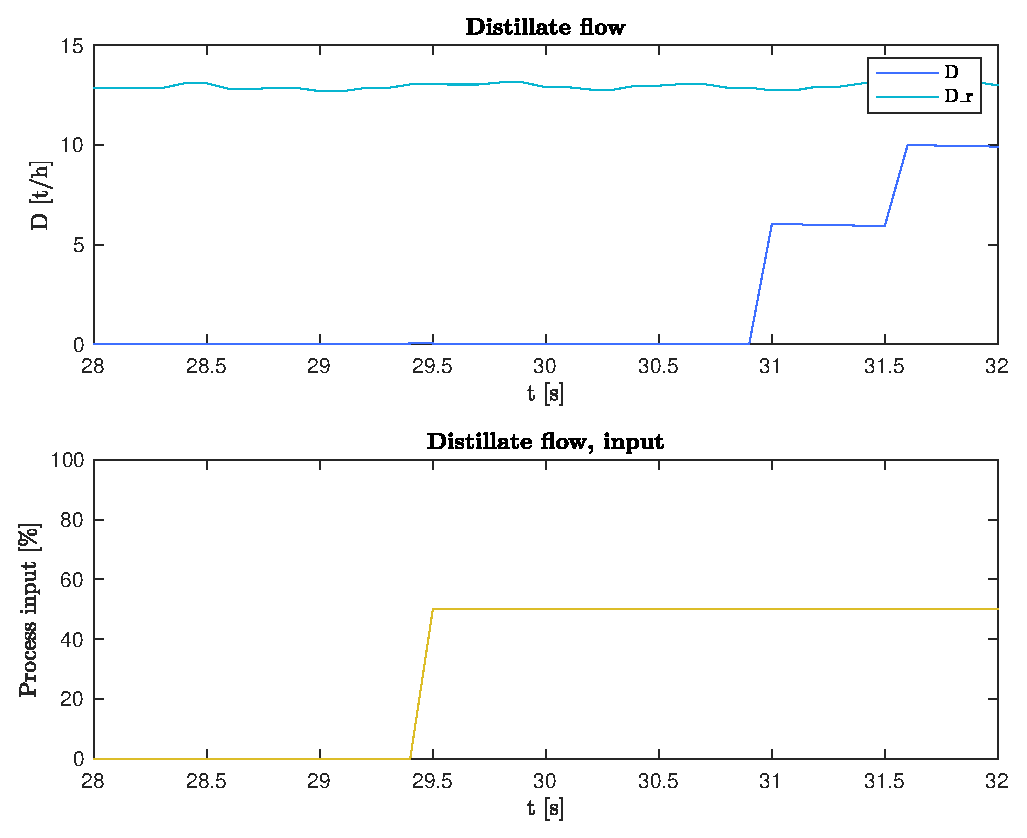
\includegraphics[width=0.8\textwidth]{../Systemanalyse/Log_Data_to_Matlab/Figurer/Stegeksperimenter/FC1005.eps}
\caption{Open-loop step response of $D$}
\label{fig:ol_step_FC1005}
\end{figure}

\begin{figure}
\centering
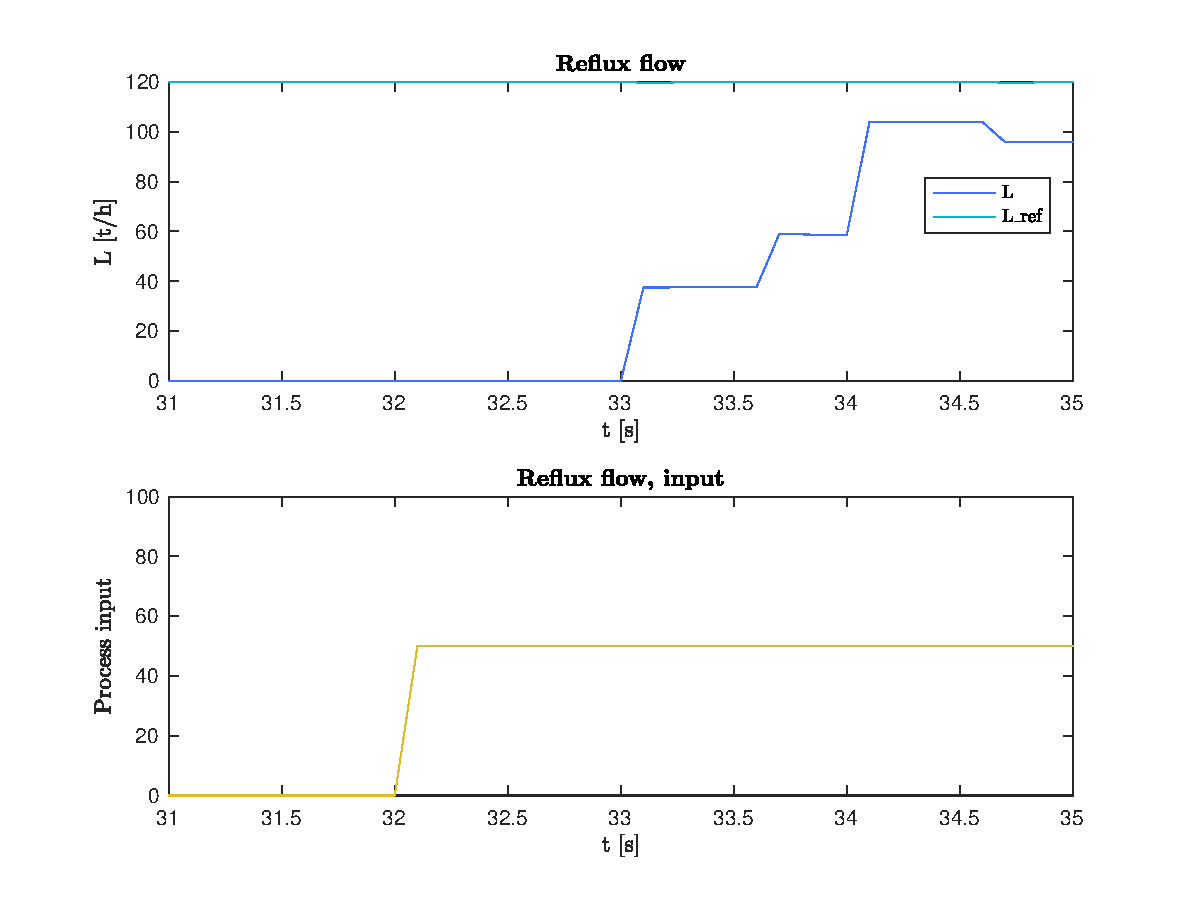
\includegraphics[width=0.8\textwidth]{../Systemanalyse/Log_Data_to_Matlab/Figurer/Stegeksperimenter/FC1015.eps}
\caption{Open-loop step response of $L$}
\label{fig:ol_step_FC1015}
\end{figure}

\begin{figure}
\centering
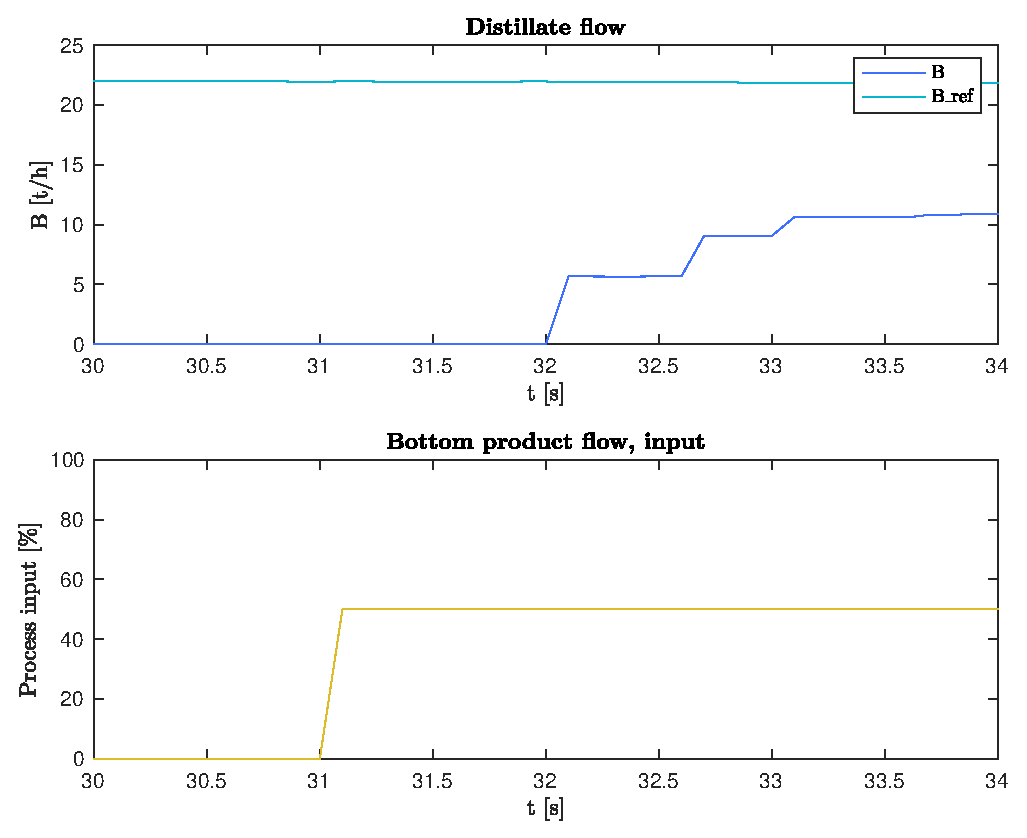
\includegraphics[width=0.8\textwidth]{../Systemanalyse/Log_Data_to_Matlab/Figurer/Stegeksperimenter/FC1019.eps}
\caption{Open-loop step response of $B$}
\label{fig:ol_step_FC1019}
\end{figure}

\begin{figure}
\centering
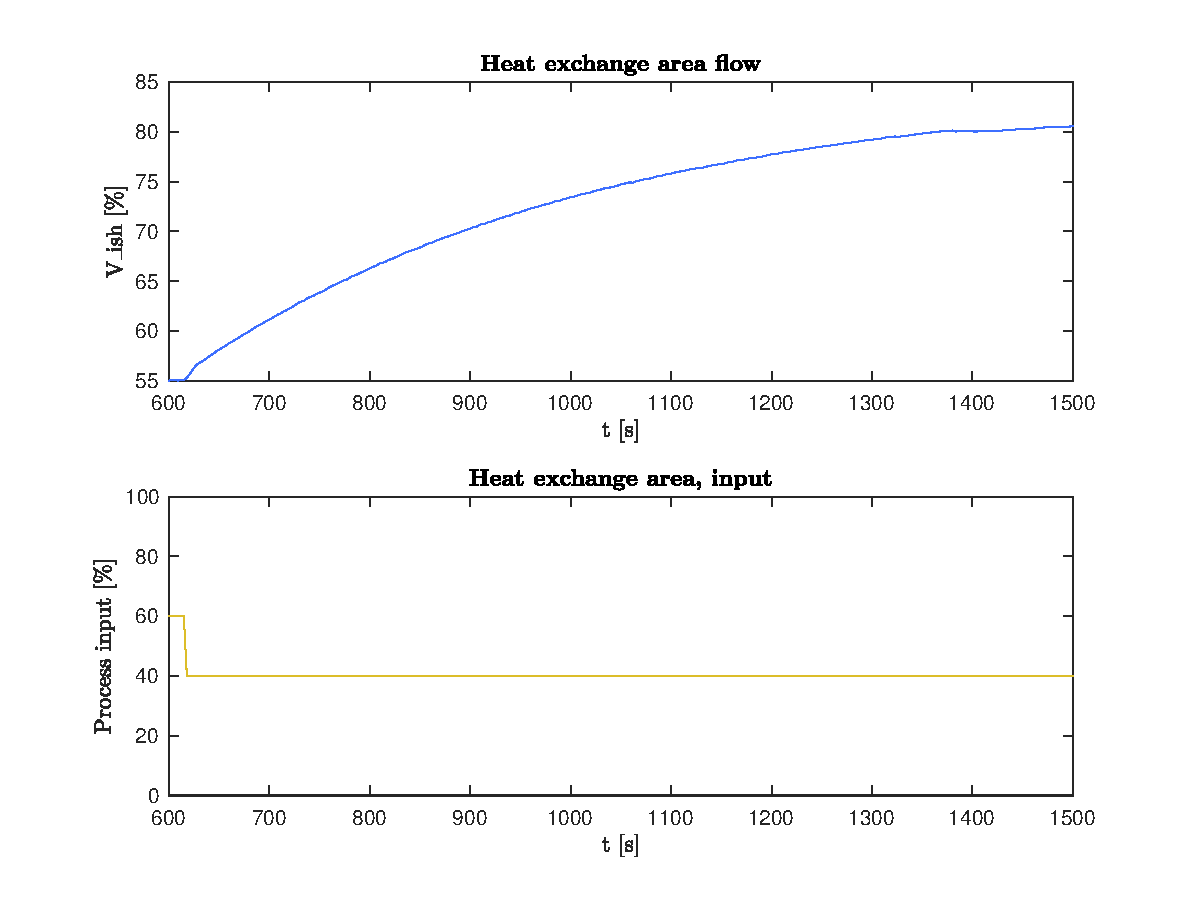
\includegraphics[width=0.8\textwidth]{../Systemanalyse/Log_Data_to_Matlab/Figurer/Stegeksperimenter/LC1028.eps}
\caption{Open-loop step response of heat exchanger area, related to $V$}
\label{fig:ol_step_LC1028}
\end{figure}

\begin{figure}
\centering
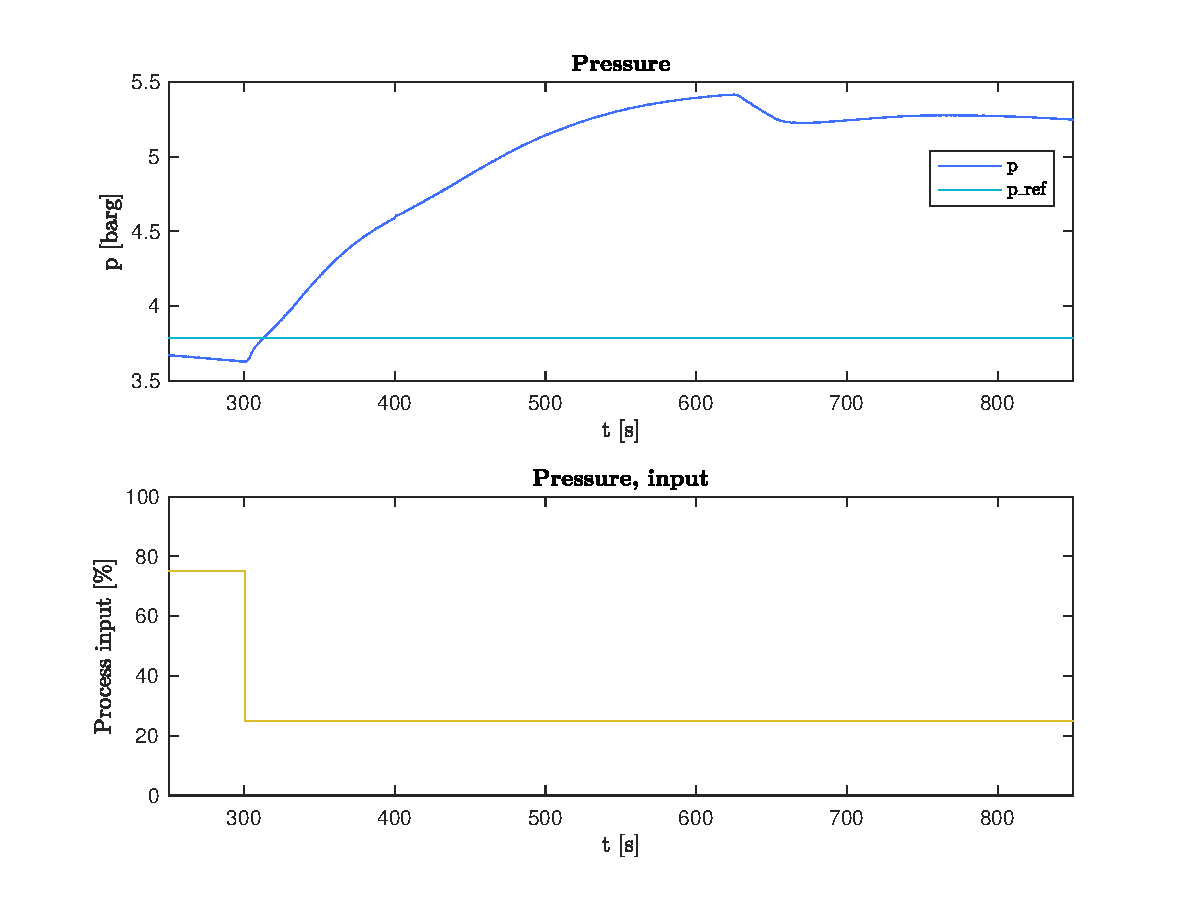
\includegraphics[width=0.8\textwidth]{../Systemanalyse/Log_Data_to_Matlab/Figurer/Stegeksperimenter/PC1024.eps}
\caption{Open-loop step response of $p$}
\label{fig:ol_step_PC1024}
\end{figure}

The data from these experiments can be seen in figures \ref{fig:ol_step_FC1005}, \ref{fig:ol_step_FC1015}, \ref{fig:ol_step_FC1019}, \ref{fig:ol_step_LC1028} and \ref{fig:ol_step_PC1024}. The accuracy of the simulations are clearly not sufficient for fitting a first order model (they behave in a stepwise fashion), but inspecting the order of magnitude of the gains and time constants is a good start. An attempt at making sense of these parameters is shown in table \ref{tab:inner_loop_step_responses}. In addition to this, a desired time constant $T_L$ is shown in the rightmost column. For a quick response, choosing $T_L = 0,3\tau$ is suggested in \cite{balchen}. Some simple trial and error showed that this lead to unfortunate between control loops, especially the controllers for $D$ and $L$. Due to this, $T_L = 2\tau$ was chosen for the three fastest control loops. Since the time delay was hard to make a meaningful reading of for the other systems, a somewhat arbitrary choice of $T_L = 10s$ was chosen for these systems. Like all the other parameters, these are not absolute choices, but a good starting point.

After calculating the SIMC controller values, some qualitative tuning was needed. Here, the integral times (which could be read decently precisely) were fixed. The resulting one degree of freedom made tuning easier, and the results of this tuning is shown in table \ref{tab:inner_loop_PI_parameters}, together with the values from the SIMC method (which were the basis for the second round of tuning). A column showing the scaled gain $G = K_p \frac{(y_{\max} - y_{\min})}{(u_{\max} - u_{\min})}$, which is the value implemented in K-spice, is also shown. The final controller gains are also given in this variable, since the parameters were changed directly in the K-spice panel. Note that $T_i$ in the $p$ control loop was changed from 40s to 20s in the final tuning.


\begin{table}
\centering
\begin{tabular}{c | c | c | c | c | c || c}
& $\tau$ & $T_1$ & $\frac{dy}{dt}$ & $\Delta u$ & $k'$ & $T_L$ \\ \hline
$D$ & 1,0s & 0,4s & 14,3 & 50\% & 28,6 & 2s \\
$L$ & 1,0s & 1,0s & 47,5 & 50\% & 95,0 & 2s \\
$B$ & 1,0s & 0,6s & 10,0 & 50\% & 20,0 & 2s \\
$V$ & $\approx$ 0 & 400s & 0,028 & 20\% & 0,14 & 10s \\
$p$ & $\approx$ 0 & 200s & 0,088 & 50\% & 0,18 & 10s
\end{tabular}
\caption{Identified parameters for inner loop}
\label{tab:inner_loop_step_responses}
\end{table}


\begin{table}
\centering
\begin{tabular}{c | c | c | c | c}
& $K_p$ & $T_i$ & $G_{\textrm{SIMC}}$ & $G_{\textrm{final}}$ \\ \hline
$D$ & 0,0035 & 0,4s & 0,42 & 0,42\\
$L$ & 0,0018 & 1,0s & 0,22 & 0,22\\
$B$ & 0,0083 & 1,0s & 1,0 & 0,30 \\
$V$ & 0,71 & 40s & 86 & 86 \\
$p$ & 0,57 & 20s & 68 & 30
\end{tabular}
\caption{PI controller parameters for inner loop}
\label{tab:inner_loop_PI_parameters}
\end{table}

\todo{Legg til noe om at resten av systemet bare var i tilfeldige tilstander med tilfeldige regulatorer.}

\newpage
\section{Level controllers}
\subsection{System identification}
\todo[inline]{Dette}
\subsection{Controller tuning}
\todo[inline]{Dette}

\newpage
\section{Composition controllers}
\subsection{System identification}
\todo[inline]{Dette}
\subsection{Controller tuning}
\todo[inline]{Dette}

\end{document}
